
\documentclass[12pt]{article}

% Layout.
\usepackage[top=1in, bottom=0.75in, left=1in, right=1in, headheight=1in, headsep=6pt]{geometry}

% Fonts.
\usepackage{mathptmx}
\usepackage[scaled=0.86]{helvet}
\renewcommand{\emph}[1]{\textsf{\textbf{#1}}}

% TiKZ.
\usepackage{tikz, pgfplots}
\usetikzlibrary{calc}
\pgfplotsset{compat = newest}
 
\pgfplotsset{my style/.append style={axis x line=middle, axis y line=
middle, xlabel={$x$}, ylabel={$y$}, axis equal }}

% Misc packages.
\usepackage{amsmath,amssymb,latexsym}
\usepackage{graphicx}
\usepackage{array}
\usepackage{xcolor}
\usepackage{multicol}

% Commands to set various header/footer components.
\makeatletter
\def\doctitle#1{\gdef\@doctitle{#1}}
\doctitle{Use {\tt\textbackslash doctitle\{MY LABEL\}}.}
\def\docdate#1{\gdef\@docdate{#1}}
\docdate{Use {\tt\textbackslash docdate\{MY DATE\}}.}
\def\doccourse#1{\gdef\@doccourse{#1}}
\let\@doccourse\@empty
\def\docscoring#1{\gdef\@docscoring{#1}}
\let\@docscoring\@empty
\def\docversion#1{\gdef\@docversion{#1}}
\let\@docversion\@empty
\makeatother

% Headers and footers layout.
\makeatletter
\usepackage{fancyhdr}
\pagestyle{fancy}
\fancyhf{} % Clears all headers/footers.
\lhead{\baselineskip 30pt
%\emph{\@doctitle\hfill\@docdate}
\emph{\@docdate\hfill\@doctitle}
\ifnum \value{page} > 1\relax\else\\
\emph{Name: \rule{3.5in}{1pt}\hfill \@docscoring}\fi}
\rfoot{\emph{\@docversion}}
\lfoot{\emph{\@doccourse}}
\cfoot{\emph{\thepage}}
\renewcommand{\headrulewidth}{0pt}%
\makeatother

% Paragraph spacing
\parindent 0pt
\parskip 6pt plus 1pt

% A problem is a section-like command. Use \problem{5} to
% start a problem worth 5 points.
\newcounter{probcount}
\newcounter{subprobcount}
\setcounter{probcount}{0}
\newcommand{\problem}[1]{%
\par
\addvspace{4pt}%
\setcounter{subprobcount}{0}%
\stepcounter{probcount}%
%\makebox[0pt][r]{\emph{\arabic{probcount}.}\hskip1ex}\emph{[#1 points]}\hskip1ex}
\makebox[0pt][r]{\emph{\arabic{probcount}.}\hskip1ex}\emph{[#1 \ifnum1=0#1\relax point\else points\fi]}\hskip1ex}
%\textbf{(#1 \ifnum1=0#1\relax thing\else things\fi
\newcommand{\thesubproblem}{\emph{\alph{subprobcount}.}}

% Subproblems are an enumerate-like environment with a consistent
% numbering scheme. 
% Use \begin{subproblems}\item...\item...\end{subproblems}
\newenvironment{subproblems}{%
\begin{enumerate}%
\setcounter{enumi}{\value{subprobcount}}%
\renewcommand{\theenumi}{\emph{\alph{enumi}}}}%
{\setcounter{subprobcount}{\value{enumi}}\end{enumerate}}

% Blanks for answers in normal and math mode.
\newcommand{\blank}[1]{\rule{#1}{0.75pt}}
\newcommand{\mblank}[1]{\underline{\hspace{#1}}}
\def\emptybox(#1,#2){\framebox{\parbox[c][#2]{#1}{\rule{0pt}{0pt}}}}

% Misc.
\renewcommand{\d}{\displaystyle}
\newcommand{\ds}{\displaystyle}
\def\bc{\begin{center}}
\def\ec{\end{center}}
\def\be{\begin{enumerate}}
\def\ee{\end{enumerate}}

\newcommand{\ans}{\rule{2 in}{.5pt}}
\newcommand{\bigans}[1]{\rule{#1 in}{.5pt}}

\doctitle{Math F251X: Quiz 1}
\docdate{January 18, 2024}
\doccourse{UAF Calculus I}
\docversion{v-1}
\docscoring{\blank{0.8in} / 25}
\begin{document}
%\textbf{Please circle your instructor's name:} \hfill Leah Berman  \hfill   Jill Faudree\\

There are 18 questions worth 25 points on this quiz. No aids (book, calculator, etc.)
are permitted.  {\bf Show all work for full credit.}

%%%Problem
\problem{1} Determine the domain and range of $f(x)=\frac{1}{x^2} + 1.$ Write your answer in interval notation. \\
\vfill
\quad \hspace{4in} \underline{\hspace{2in}}

%%%Problem
\problem{1} For $f(x)=8 - x^2$ and $g(x)=2-x$, find the composition $f \circ g$ and simplify your answer.\\
\vfill
\quad \hspace{4in} \underline{\hspace{2in}}

%%%Problem
\problem{1} Write the expression $\frac{x^7y^4z}{x^3y^{-1}z^3}$ in the form $x^ay^bz^c$. That is, write the expression with all terms in the numerator. 	\\
\vfill
\quad \hspace{4in} \underline{\hspace{2in}}

%%%Problem
\problem{1} A rectangle has length $\ell$ that is twice its width, $w$. Find an expression for the area, $A$, of the rectangle in terms of its width, $w.$\\
\vfill
\quad \hspace{4in} \underline{\hspace{2in}}

%%%Problem
\problem{2} Write an equation of the line between the points $(-4,5)$ and $(2,1).$ \\

\vfill

\quad \hspace{4in} \underline{\hspace{2in}}\\

\vfill

Is the line increasing, decreasing, horizontal or vertical.\hfill \underline{\hspace{2in}}\\

\newpage

%%%Problem
\problem{1} Simplify the expression $\frac{2x^3+2x^2y}{4x^2+12xy}$ by cancelling any common factor in both the numerator and denominator.\\
\vfill
\quad \hspace{4in} \underline{\hspace{2in}}

%%%Problem
\problem{2} Sketch the graph of $f(x)= 4-x^2.$ Label any $x$- or $y$-intercepts in your sketch.\\

\begin{tikzpicture}[scale=0.7]
\draw[->](-4,0)--(4,0);\draw[->](0,-4)--(0,4);
\end{tikzpicture}
\vfill
\quad \hspace{2in} asymptote(s)? \underline{\hspace{2in}} \\

%%%Problem
\problem{2} Use the piecewise defined function $\displaystyle f(x)=\begin{cases} \frac{x}{x-1} & x \leq 0 \\ \sqrt{x} & x>0 \end{cases}. $\\
	\begin{subproblems}
	\item Find $f(-1).$ \hfill \underline{\hspace{2in}}\\
	\vfill
	\item Determine $x$ such that $f(x)=4.$ \hfill \underline{\hspace{2in}}\\
	\vfill
	\end{subproblems}

%%%Problem
\problem{1} Evaluate $\cos(4\pi/3)$ exactly.\\
\vfill
\quad \hspace{4in} \underline{\hspace{2in}}

%%%Problem
\problem{1} Solve the equation $\sin(x)+1=0$ on the interval $0 \leq x < 2\pi.$\\
\vfill
\quad \hspace{4in} \underline{\hspace{2in}}

\newpage

%%%Problem
\problem{1} In the right triangle below, $a=4$ and $c=5.$ Determine the value of $\tan(A)$, the tangent function at angle $A.$ 
	
	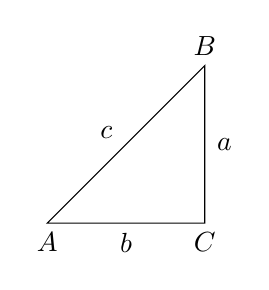
\begin{tikzpicture}[scale=0.5]
	\draw (0,0) node[anchor=north]{$A$}
  -- (4,0) node[anchor=north]{$C$}
  -- (4,4) node[anchor=south]{$B$}
  -- cycle;
  	\node at (2,-0.5){$b$}; \node at (4.5,2){$a$}; \node at (1.5,2.3){$c$};
	\end{tikzpicture}\\
\vfill
\quad \hspace{4in} \underline{\hspace{2in}}
%%%Problem
\problem{2} Sketch the graph of $f(x)=e^{-x}+1$. Label any $x$- or $y$-intercepts. Give the equation of any asymptotes of $f(x).$\\
\begin{tikzpicture}[scale=0.7]
\draw[->](-4,0)--(4,0);\draw[->](0,-3.5)--(0,4);
\end{tikzpicture}
\vfill
\quad \hspace{2in} asymptote(s)? \underline{\hspace{2in}}
%%%Problem
\problem{1} Solve the equation $18-4^x=10.$\\
\vfill
\quad \hspace{4in} \underline{\hspace{2in}}

%%%Problem
\problem{2} Sketch the graph of $f(x)=\ln(x+1)$. Label any $x$- or $y$-intercepts. Give the equation of any asymptotes of $f(x).$\\
\begin{tikzpicture}[scale=0.7]
\draw[->](-4,0)--(4,0);\draw[->](0,-4)--(0,3.5);
\end{tikzpicture}
\vfill
\quad \hspace{2in} asymptote(s)? \underline{\hspace{2in}} \\

\newpage

%%%Problem
\problem{1} Solve the equation $\displaystyle \frac{\ln(x-1)}{3}=4.$\\
\vfill
\quad \hspace{4in} \underline{\hspace{2in}}

%%%Problem
\problem{1} Solve the inequality $x^2 \geq 9.$ Write your answer in interval notation.\\
\vfill
\quad \hspace{4in} \underline{\hspace{2in}}

%%%Problem
\problem{2}Sketch the graph of $f(x)=3\cos(x)$ on  the interval $0 \leq x \leq 2\pi.$ Label any $x$- or $y$-intercepts. Give the equation of any asymptotes of $f(x).$\\
\begin{tikzpicture}[scale=0.7]
\draw[->](-4,0)--(4,0);\draw[->](0,-4)--(0,4);
\end{tikzpicture}
\vfill
\quad \hspace{2in} asymptote(s)? \underline{\hspace{2in}} \\
 \\

%%%Problem
\problem{2} Use the graph of $f(x)$ below to answer the questions.\\

\begin{minipage}{.4\textwidth}
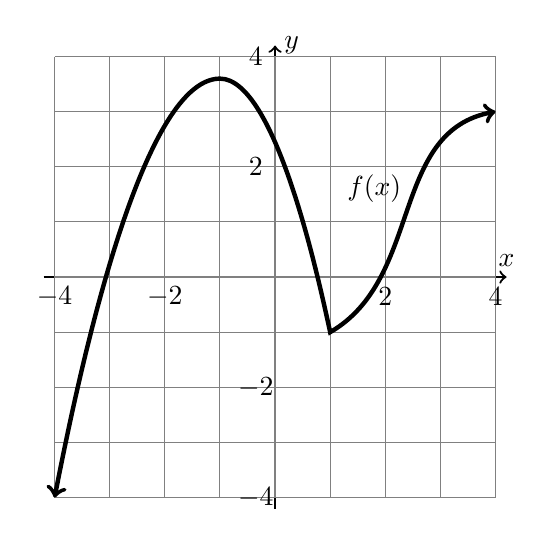
\begin{tikzpicture}[scale=.7]
\draw[thick, ->] (-4.2,0) -- (4.2,0);\draw[thick, ->] (0,-4.2) -- (0,4.2);
\node at (4.2,.3){$x$}; \node at (.3,4.2){$y$};
\foreach \i in {-4,-3,...,4}{
	\draw[gray] (-4,\i) -- (4,\i); \draw[gray] (\i,-4) -- (\i,4);

	}
\foreach \i in {-4,-2,2,4}{
	\node at (\i,-.35){$\i$};
	\node at (-.35,\i){$\i$};
	}
\node at (1.8, 1.6) {$f(x)$};
%\draw[ultra thick] (-1,0) -- (1,2) -- (2,-2);	
%\filldraw (-1,0) circle (3pt); \filldraw (2,-2) circle (3pt);

\draw[ultra thick, <->] (4, 3) to[in = 30, out = 190] (1,-1) parabola bend (-1, 3.6) (-4,-4);

%\node at (-1,-.3){$-2$};\node at (1,-.3){$2$};\node at (2,-.3){$4$};\node at (3,-.3){$6$};
%\node at (-.3,-1){$-1$};\node at (-.3,1){$1$};\node at (-.3,2){$2$};\node at (-.3,3){$3$};
\end{tikzpicture}
\end{minipage}
\begin{minipage}{.6\textwidth}
	\begin{subproblems}
	\item {\bf Estimate} $f(0)$. \hfill \ans 
	\vspace{12 pt}
	\item {\bf Estimate} an $x$-value such that $f(x)=-2.$ 
	\vspace{12 pt}
	
	\hfill \ans
	\end{subproblems}
\end{minipage}	






\end{document}